\chapter{NC-Aggregate}



NCAs sind seit einigen Jahren ein neu hinzugekommener, selbst entwickelter Teil des Bihler Baukastensystems zur Massenfertigung von Präzisionsteilen auf deren Stanz-, Biege- und Umformautomaten. \cite{OttoBihlerMaschinenfabrikGmbH&Co.KG2012} Innerhalb dieses Systems dienen sie dazu, Werkzeugbewegungen schnell und exakt auszuführen, d.h. sie stellen hohe Kräfte und schnelle Bewegungen bereit.



Parallel dazu werden auf anderen Maschinen auch noch die in früheren Jahren entwickelten über Kurvenscheiben gesteuerten Schlittenaggregate verwendet. Diese rein mechanisch gesteuerten Maschinen sind sehr robust und zuverlässig. Auch können mit ihnen sehr hohe Produktionsgeschwindigkeiten erreicht werden. Ihre Stärke liegt in der Produktion hoher Losgrößen, wo beständig große Mengen gleicher Teile hergestellt werden sollen. Die Rüstzeiten bei einem Werkzeugwechsel sind dagegen lang und wenn es, wie zumeist von der heutigen Wirtschaft gefordert, darum geht, die Lagerbestände gering zu halten und die entsprechenden Teile zum geforderten Termin zu liefern, dann haben die NC-Systeme entscheidende Vorteile.


Aus der Kombination von Mechanik, Elektrotechnik und Informatik ergeben sich für die NCAs im Vergleich zu den klassischen mechanisch angetriebenen Schlittenaggregaten folgende Vorteile: \cite{OttoBihlerMaschinenfabrikGmbH&Co.KG2012} 

\begin{itemize}
 \item Der Wechsel von mechanischen Komponenten beim Rüsten wird deutlich reduziert.
 \item Die Rüstzeit ist sehr kurz.
  \item Verschiedene Prozesse können schnell und einfach reproduziert werden. 
 \item Verschiedenste Prozesse können auf einer Anlage kombiniert und integriert werden.
 \item Hubbewegungen und Bewegungsprofile sind frei programmierbar.
 \item Der Umgang mit dem Werkstoff ist wegen der freien Programmierbarkeit der Fahrprofile sehr schonend.
 \item Die Maximalkraft ist über den gesamten Arbeitsbereich frei wählbar.
 \item Eine Kraftsteuerung ist möglich.
\end{itemize}






Insbesondere mit der neuen Maschinengeneration GRM-NC und RM-NC werden die Vorteile der NC-Technik ausgenutzt. Eine der Kernkomponenten dieser Maschinen sind die NCAs. Durch die derzeitig hohe Nachfrage nach diesen Maschinen ist auch die benötigte Stückzahl der NCAs stark gestiegen.





\section{Beschreibung der NC-Aggregate} \label{cha:Beschreibung_der_NCAs}


Die NC-Aggregate sind komplexe Bauteile, die viele, sehr präzise gefertigte, genau aufeinander abgestimmte Komponenten enthalten. In Abbildung~\ref{fig:NCA_Mit_Beschriftung} sind wichtige Details des Aufbaus schematisch dargestellt. Nicht aus der Darstellung ersichtlich ist, dass sie darüber hinaus noch Dichtungen, Gleitsteine, Versorgungsbohrungen für Kühlung und Schmierung und je nach Bauart ein Linearmesssystem  enthalten.


\begin{figure}[H]
\centering
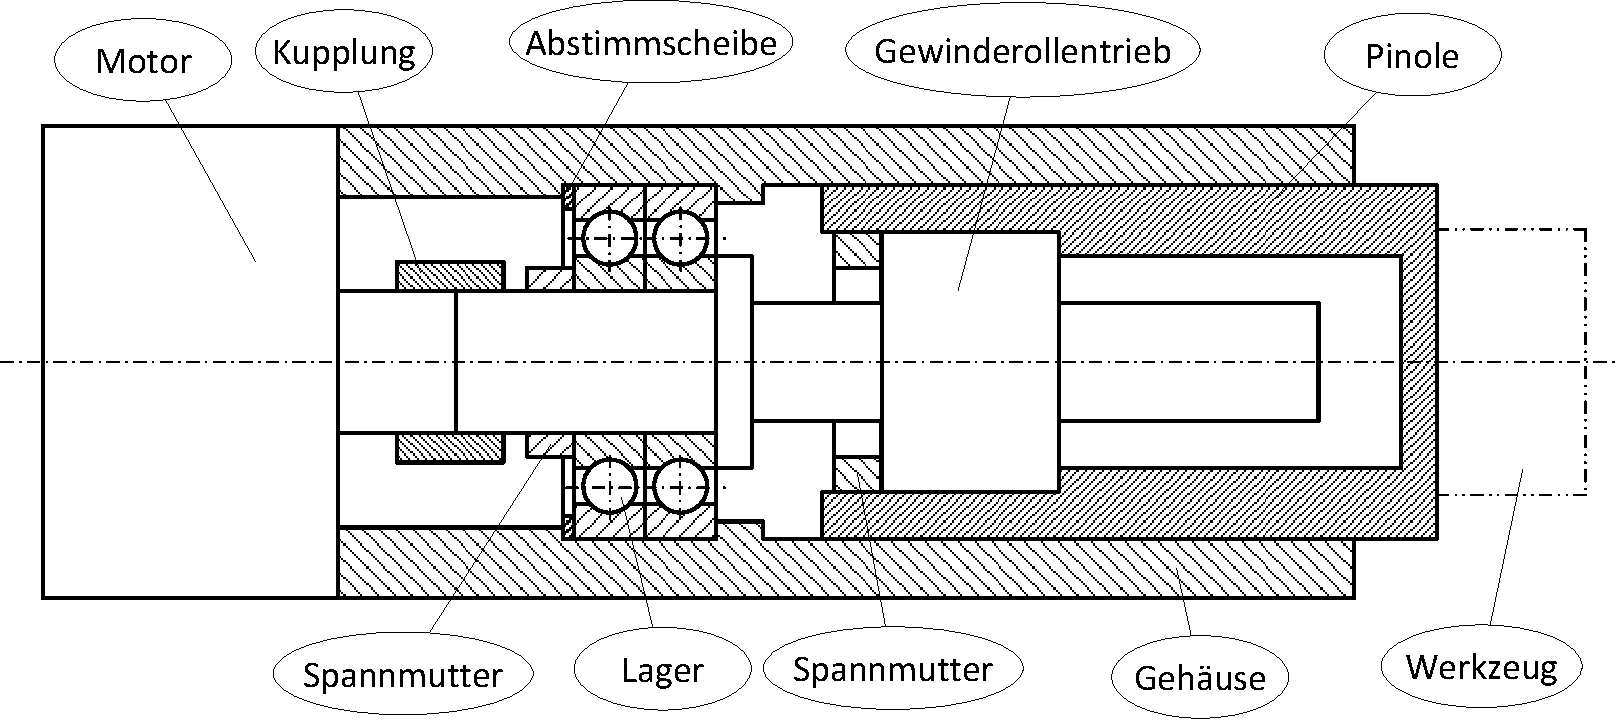
\includegraphics[width=\textwidth]{NC_Aggregat_Skizze1_mit_Beschriftung_und_Werkzeug} % Skizze von der Funktionsweise der NC Aggregate
\caption{Schematische Darstellung eines NC-Aggregats}
\label{fig:NCA_Mit_Beschriftung}
\end{figure}


Um die notwendige Arbeit zu verrichten, treibt der Elektromotor über eine Kupplung einen Gewinderollentrieb an. Die Mutter des Gewinderollentriebes versetzt die Pinole in eine axiale Bewegung. An die Pinole kann, wie in Abbildung~\ref{fig:NCA_Mit_Beschriftung} dargestellt, ein Werkzeug montiert werden. Das Werkzeug wird durch die Bewegung der Pinole linear angetrieben.



\subsection{Mechanischer Aufbau}

Die Spindel des Gewinderollentriebes ist über Schrägkugellager im Gehäuse gelagert und mit einer Spannmutter gesichert. Die Mutter des Gewinderollentriebes ist mit der Pinole über eine Passfeder und eine Spannmutter verbunden. Zur Verdrehsicherung sind in der Pinole zwei Gleitsteine befestigt, die im Gehäuse laufen. Je nach Variante ist ein Messlineal auf der Pinole oder einem Gleitstein befestigt. Der entsprechende Messkopf befindet sich im Gehäuse.

\subsection{Elektrische Komponenten}\label{cha_Elektrische_Komponenten}

Die verwendeten Elektromotoren sind Synchronmotoren. Als Messsystem für die Steuerung stehen der Motorgeber EQN 1325-2048 von Heidenhain und bei den NCA 4 und 5 Modellen zusätzlich ein direktes Wegmesssystem in Form eines Messlineals zur Verfügung.


% Als Motorgeber wird bei allen NCA der Drehgeber EQN 1325-2048 von Heidenhain benutzt.

%Diese baulichen Unterschiede sind bei der Steuerung der NCAs von Bedeutung. Hierbei wird zwischen zwei grundsätzlich unterschiedlichen Regelungsarten unterschieden. Diese werden im Hause Bihler als Ein- und Zweigeberregelung bezeichnet.


%Bei der Eingeberregelung wird der Motordrehgeber als Messsystem für die Regelung benutzt. Hierbei wird die axiale Position der Pinole indirekt über die rotatorische Position des Motors geregelt.

%Bei der sogenannten Zweigeberregelung wird die axiale Position der Spindel über das lineare Wegmesssystem geregelt. Hierdurch ist eine wesentlich höhere Genauigkeit bei der Pinolenposition möglich als bei der Eingeberregelung. Der Motordrehgeber regelt hier die Position nicht, aber die Daten aus dem Motordrehgeber werden  zur Absicherung der Aggregate benutzt. So wird die Maschine gestoppt, wenn die axiale Position zu weit von der rotatorischen Position abweicht.



\subsection{Steuerung}\label{cha_Steuerung_Aufbau_NCA}

Die Regelung des Motors wird von einem ACOPOSmulti Regler der Firma B \& R übernommen. Die Bedienung erfolgt über die \gls{VC1} Steuerung der Firma Bihler.


Zum exakten Steuern der Pinole sind die NCAs verschieden aufgebaut (siehe Kapitel~\ref{cha_Elektrische_Komponenten}). Diese baulichen Unterschiede sind bei der Steuerung der NCAs von Bedeutung. Hierbei wird zwischen zwei grundsätzlich unterschiedlichen Regelungsarten unterschieden. Diese werden im Hause Bihler als Ein- und Zweigeberregelung bezeichnet. Bei der Eingeberregelung wird der Motordrehgeber als Messsystem für die Regelung benutzt. Hierbei wird die axiale Position der Pinole indirekt über die rotatorische Position des Motors geregelt. Bei der sogenannten Zweigeberregelung wird die axiale Position der Spindel über das lineare Wegmesssystem geregelt. Hierdurch ist eine wesentlich höhere Genauigkeit bei der Regelung der Pinolenposition möglich als bei der Eingeberregelung. Der Motordrehgeber regelt in diesem Fall die Position nicht, aber die Daten aus dem Motordrehgeber werden  zur Absicherung der Aggregate benutzt. So wird die Maschine gestoppt, wenn die axiale Position zu weit von der rotatorischen Position abweicht.



\subsection{Weitere Komponenten}\label{cha:Kuelkreislauf_Schmierkreislauf}

Außer den für jedes einzelne Aggregat benötigten Komponenten sind zum Betrieb der Aggregate noch ein Kühlmittelkreislauf und eine Schmiermittelversorgung notwendig, die für mehrere Aggregate gleichzeitig zur Verfügung stehen.

Das Schmieröl CGLP 220 wird über die Zentralschmierung der Maschine zu den einzelnen NCAs gefördert. Es handelt sich um eine Verbrauchsschmierung. Dabei gelangt das Schmieröl aus einem Vorratsbehälter mithilfe einer Pumpe über Verteiler zu den einzelnen NCAs. Die Zuteilung zu den verschiedenen zu schmierenden Bereichen erfolgt über Zumessventile. Die Förderung des Öls erfolgt nicht kontinuierlich sondern stoßweise in Impulsen. Das zudosierte Schmiervolumen pro Impuls ist durch die verwendeten Zumessventile festgelegt. 

\section{Unterschiede der NC-Aggregate}\label{cha:Unterschiede der NC-Aggregate}

Die Firma Bihler bietet zur Zeit 11 Standardvarianten der NC-Aggregate an. Im Moment werden hauptsächlich die Größenvarianten NCA 2 bis NCA 5 verwendet. Aufgrund der unterschiedlichen Anforderungen im Einsatz benötigt man diese verschiedenen Varianten der NCAs, die grundsätzlich nach demselben Schema (vergleiche Abbildung~\ref{fig:NCA_Mit_Beschriftung}) konzipiert sind. Der wichtigste Unterschied ist hierbei die Kraft, die die NCAs zur Verfügung stellen. Die Kraft hängt maßgeblich von der Größe der NCAs ab. Die Punkte, in denen sich die NCAs hauptsächlich unterscheiden, sind in Abbildung~\ref{fig:Unterschiede_der_NCA_Varianten} aufgeführt.



Neben der Größe kann auch die Spindelsteigung des Rollengewindetriebes variiert werden. Dies führt zu anderen Übersetzungen, was die Spitzenkraft bei sonst gleichen Randbedingungen ändert. Allerdings ist hierbei zu beachten, dass sich die Spitzenkraft indirekt proportional zur maximalen Verfahrgeschwindigkeit verändert.  Deshalb muss bei einer Anforderung an eine höhere Kraft von einer Einbuße an Geschwindigkeit ausgegangen werden.

Darüber hinaus ist für viele Anwendungen der maximale Verfahrweg interessant. Aus diesem Grund gibt es je nach Bedarf Aggregate mit den passenden Hublängen. Bei besonders großen Hublängen nimmt die Steifigkeit der Aggregate ab.


Außer in mechanischen Kriterien unterscheiden sich die Aggregate auch durch die verwendeten elektrischen Komponenten. Dabei handelt es sich um die Gebersysteme. Bei der Firma Bihler kommen zwei Gebersysteme zum Einsatz. Beim 1-Geber-System erfolgt die Regelung der Achse nur über den Motorgeber. Bei dem 2-Geber-System ist zusätzlich zu dem Motorgeber noch ein lineares Messsystem verbaut.

NCA 2 und NCA 3 sind derzeit als 1-Geber-System ausgeführt. NCA 4 und NCA 5 sind als 2-Geber-System ausgeführt. Dies wurde notwendig, da durch die Temperaturdehnung und der damit verbunden geringen Positioniergenauigkeit der Achse eine Regelung nur mit dem Motorgeber nicht die erwarteten Toleranzen erfüllt. Aus diesem Grund wurde bei den NCA 4 und NCA 5 ein lineares Messsystem auf der Pinole eingebaut. Auch bei den NCA 2 und NCA 3 gibt es derzeit Überlegungen, die auf den Einbau eines solchen Messsystems abzielen.

Bei den NCA 4 ist das Messlineal auf der Pinole aufgeklebt. Es wird ein magnetisches Wegmesssystem der Firma Balluf verwendet. Es kommt das Messsystem BML-S1H1-B6QC-M3CA-D0-KA00,8-ZA17 zum Einsatz.

Bei den NCA 5 ist das Messlineal auf dem Gleitstein aufgeklebt. Es wird ein induktives Wegmesssystem der Firma AMO verwendet. Es kommt das Messsystem  LMKA-11100.113-0,8-9-S28 zum Einsatz.


\begin{table}[H]
\center
\fbox{
\begin{minipage}[c]{0.6\textwidth}
\vspace{5pt}
\begin{itemize}
 \item Mechanisch
 \begin{itemize}
    \item Größe
    \item Spindelsteigung des Rollengewindetriebes
    \item Maximaler Hub
 \end{itemize}
 \item Elektrisch
 \begin{itemize}
    \item Gebersystem
    \item Motor
 \end{itemize}
\end{itemize}
\par\vspace{2pt}
\end{minipage}}
\caption{Unterschiede der NCA Varianten}
\label{fig:Unterschiede_der_NCA_Varianten}
\end{table}




In Tabelle~\ref{tab:Übersicht_über_die Unterschiede_der_Verschiedenen_NCA_Varianten} sind die Unterschiede der derzeit als Standard etablierten NCAs aufgeführt. Eine Komplettübersicht über die  Kenngrößen dieser NCAs findet sich im Anhang~\ref{cha_Anhang_4}. Die Daten entstammen der Arbeit von Riedle \cite{Riedle2015}. 


\begin{table}[h]
\centering



\resizebox{\textwidth}{!}{%
\begin{tabular}{cccccc}\toprule
Aggregat Sach-Nr. & Aggregat & Max. Hub & 2-Geber-System & Motor Sach-Nr. & Steigung \\
 & Beschreibung & mm &  &  & mm/Umdr \\
 \midrule
100-54-0575.0 & NCA 2 / 60.5000 & 60 & nein & 907-74-0762.5 & 5 \\
100-54-0580.0 & NCA 2 / 120.5000 & 120 & nein & 907-74-0762.5 & 5 \\
100-54-0585.0 & NCA 2 / 60.1500 & 60 & nein & 907-74-0762.5 & 16 \\
100-54-0590.0 & NCA 2 / 120.1500 & 120 & nein & 907-74-0762.5 & 16 \\
100-54-0592.0 & NCA 2 / 240.1500 & 240 & nein & 907-74-0762.5 & 16 \\
100-54-0720.0 & NCA 3 / 120.8900 & 120 & nein & 907-74-0749.5 & 10 \\
100-54-0730.0 & NCA 3 / 200.3500 & 200 & nein & 907-74-0749.5 & 25 \\
100-54-0632.0 & NCA 4 / 120.12000 & 120 & ja & 907-74-0741.5 & 16 \\
100-54-0700.0 & NCA 4 / 120.19000 & 120 & ja & 907-74-0741.5 & 10 \\
100-54-0635.0 & NCA 5 / 100.31000 & 100 & ja & 907-74-0745.5 & 15 \\
100-54-0637.0 & NCA 5 / 100.47000 & 100 & ja & 907-74-0745.5 & 10 \\
\bottomrule
\end{tabular}
}
\caption{Übersicht über die Unterschiede der verschiedenen NCA Varianten}
\label{tab:Übersicht_über_die Unterschiede_der_Verschiedenen_NCA_Varianten}
\end{table}



% mithilfe der Stanz-Biegewerkzeuge, die mit einem Spannbolzen an der Pinole des NC-Schlittenaggregats befestigt sind, können Bearbeitungsschritte am Band vorgenommen werden. Die Bestandteile wie das Gehäuse, die Pinole, der AC-Servomotor, der Flansch, das Kopflager, die Gleitsteine und der Rollengewindetrieb sowie der Aufbau sind in Bild 3.16 genauer beschrieben.


% Der AC-Servomotor mit Kühlmantel und indirekter Spindelkühlung ist über einen Flansch mit dem Gehäuse des Aggregats verbunden. Die vom Motor erzeugte Rotation wird über einen Rollengewindetrieb in eine lineare Hubbewegung der Pinole umgewandelt. Gleitsteine, die in der Pinole befestigt und im Gehäuse geführt sind, gewährleisten diese rein translatorische Bewegung. Somit lassen sich Kräfte von 400 N bis 38 KN erzeugen, die an jeder beliebigen Hubposition vollständig zu Verfügung stehen. Mit einem verstärkten Kopflager können sogar kurzzeitige Spitzenkräfte von doppelter Nennkraft erreicht werden. Damit bei diesen Spitzenleistungen Temperaturausdehnungen keinen Einfluss auf den Prozess haben, können diese durch ein Modell oder ein Linear-Gebersystem kompensiert werden. Eine Kraftsteuerung durch einstellbare Momentbegrenzung am Antrieb bei der Programmierung eines Überhubs ermöglicht eine optimale Prozesssicherheit.




\section{Besonderheiten der Bauelemente}\label{cha_Besonderheiten_der_Bauelemente}

Vor dem Betreiben der NCAs in der Produktion sind einige Besonderheiten zu beachten.

So können die Gewinderollentriebe nach der Fertigung nicht direkt voll belastet werden. Um einen sicheren Betrieb zu gewährleisten, müssen diese erst einige Zeit unter geringer Last gefahren werden, das heißt man lässt sie einlaufen. Hierbei werden die Gewindeflanken geglättet. Ohne diese Einlaufphase erhitzt sich der Gewinderollentrieb bei starker Belastung. Dies führt zu einer verminderten Lebensdauer des Gewinderollentriebes. Bei der Firma SKF  können bereits eingelaufene Gewinderollentriebe erworben werden. Diese haben dann bereits 20.000 Hübe absolviert. \cite{SKFGroup2014} Ansonsten empfiehlt SKF die Gewinderollentriebe vor der Verwendung einlaufen zu lassen.  Weitergehende Untersuchungen zum Einlaufprozess sind nicht bekannt.




Außerdem muss das Messsystem des NCA 4 vor der Benutzung kalibriert werden. Es handelt sich hierbei um das magnetische Messsystem der Firma Balluf. \cite{BalluffConfigurationtool} Die sogenannte Kalibrierroutine dient der Verifizierung des Gesamtsystems. Hierfür wird das NCA 4 nach der Montage auf dem Teststand aufgebaut. Das Messlineal wird an die Prüfvorrichtung angeschlossen. Der komplette Verfahrweg wird dann im Eingebersystem abgefahren. Nachdem das Gesamtsystem verifiziert ist, wird der normale Testablauf gefahren.






\section{Grundlagen der Bewegungsprofile}\label{cha:Steuerung_der_Achsen}

% Um zu verstehen, welche vielfältigen Möglichkeiten es gibt, die NC-Achsen einzusetzen, soll nachfolgend die Ansteuerung der Achsen mit der \gls{VC1} Steuerung beschrieben werden.

Um zu verstehen, welche vielfältigen Möglichkeiten es gibt, die NC-Achsen einzusetzen, ist es erforderlich, zu wissen,  wie die Ansteuerung der Achsen mit der \gls{VC1} Steuerung erfolgt. Die allgemeinen Grundlagen hierfür sind das Funktionsprinzip des Kurvengetriebes und die Verfahrbewegungen Trapez- und Dreiecksprofil. Die konkrete Umsetzung dieser Prinzipien in der VC 1 Steuerung erfolgt mit sogenannten synchronen und asynchronen Bewegungen.


% Die aus den verschiedenen Bewegungsmöglichkeiten gewählte Bewegung wird in Bewegungsprofilen mit der Vario Control 1 festgeschrieben. 
%Die Bewegungsprofile, nach denen die Pinole der NCAs bewegt wird werden bei der Firma Bihler mithilfe der VC 1 Steuerung erstellt.


%\section{Allgemeine Grundlagen}


\subsection{Funktionsprinzip Kurvengetriebe}\label{cha:Funktionsprinzip Kurvengetriebe}


Bei den mechanisch gesteuerten Maschinen wird über den Hauptantrieb das Großrad angetrieben, das Kurvenscheiben antreibt. So wird die Drehbewegung des Antriebes mit einem geradlinig geführten Abtriebsglied in eine translatorische Bewegung umgesetzt um z.B. einen Umformvorgang auszuführen. Diese miteinander verbundenen Maschinenelemente werden als Kurvengetriebe bezeichnet. Das Kurvengetriebe kann mithilfe der Getriebelehre als Modell betrachtet und berechnet werden. Mit analytischen Funktionen (sogenannten Bewegungsgesetzen) kann die Relativbewegung von zwei Getriebegliedern beschrieben werden. Als Funktion für die Antriebsbewegung wird der zeitabhängige Antriebsdrehwinkel $\varphi(t)$ verwendet. Die Abtriebsbewegung wird bei den hier translatorisch geführten Abtriebsgliedern durch den Verlauf des Abtriebsweges $s[\varphi(t)]$ beschrieben. Eine graphische Darstellung der Größen kann der Abbildung~\ref{fig:Kurvengetriebe_Funktionsbild} \cite{VDI2002} entnommen werden. 

\begin{figure}[h]
\centering
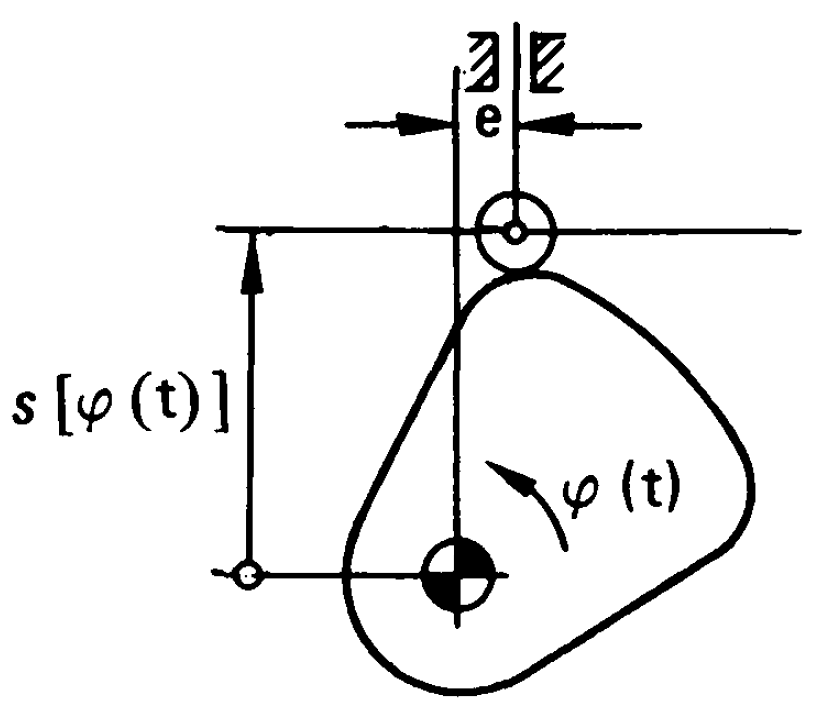
\includegraphics[width=0.3\textwidth]{Kurvengetriebe_Zuordnung_2} 



\caption{Darstellung der Einheiten am Kurvengetriebe} 
\label{fig:Kurvengetriebe_Funktionsbild}
\end{figure}

Wenn die Winkelgeschwindigkeit des Antriebsgliedes konstant bleibt, kann ein sich zyklisch wiederholender Bewegungsablauf als Funktion des Weges über die \SI{360}{\degree} eines Kreises aufgetragen werden. Für eine gegebene Rotationsgeschwindigkeit (z.B. Maschinendrehzahl) des Antriebsgliedes können die Winkelgrößen in Zeitgrößen umgerechnet werden. 














\subsection{Trapez- und Dreiecksprofil} \label{cha:Trapez und Dreiecksprofil}

%\colorbox{yellow}{nochmal Formel Zeichen anschauen}

Bei der Fahrbewegung im Trapezprofil steigt die Geschwindigkeit konstant an bis die Zielgeschwindigkeit erreicht ist. In der Abbremsphase nimmt die Geschwindigkeit konstant ab. Wenn man die Geschwindigkeit über die Zeit aufträgt, entsteht eine trapezförmige Kurve. (vgl. Abbildung~\ref{fig:Trapezprofil})  

Ein Trapezprofil ergibt sich auch unter dem Aspekt der Drehzahl, wenn sie sich während der Beschleunigungs- und der Bremsphase konstant verändert. \cite{Kiel2007a} Zwischen der Beschleunigungs- und der Bremsphase wird wiederum ein Bereich mit konstanter Maximalgeschwindigkeit erreicht.

Solange keine äußeren Kräfte auf das System wirken, sind die Beschleunigung und das Drehmoment direkt proportional. Da die Spannung im Motor konstant gehalten wird, sind der Motorstrom und das Drehmoment direkt proportional. Dies bewirkt, dass der Verlauf der Kurven von Beschleunigung, Drehmoment und Motorstrom gleich sind.





\begin{figure}[h]









\begin{tikzpicture}
\begin{groupplot}[
        group style={
            group size=1 by 2,
            xlabels at=edge bottom,
            ylabels at=edge left,
            xticklabels at=edge bottom,
            vertical sep=3pt,
            % vertical sep=40pt
        },
 	width=\textwidth,
 	height=0.2\textheight,
 	xmin=0,
 	xmax=360,
 	xtick={0,60,...,360},
 	xlabel={Winkel in $^\circ$},
 	yticklabel style = {font=\small,xshift=0.25ex},
 	,
 	ylabel style = {font=\small,xshift=0.25ex},
    ]
    
    
    
\nextgroupplot [
 	no markers,
 	ymin=0,
    ymax=50,
    %ytick={},
  	%title=Einfahrzyklus Drehmomentprofil,
    ylabel={Geschwindigkeit},
    grid=major,
    %
    %legend entries={Temperatursensor 1,Temperatursensor 2,Temperatursensor 3},
    %legend pos=south east,
    %enlarge x limits=0.01,
]
 	\addplot coordinates { 
 	    (0,0)
 	    (60,0)
 	    (120,40)
 	    (180,40)
 	    (300,0)
 	    (360,0)
    };



\nextgroupplot [
 	no markers,
 	ymin=-1,
    ymax=1,
    ytick={-1,-0.5,...,0.5},
  	%title=Einfahrzyklus Drehmomentprofil,
    ylabel={Beschleunigung},
    grid=major,
    %legend entries={Temperatursensor 1,Temperatursensor 2,Temperatursensor 3},
    %legend pos=south east,
    %enlarge x limits=0.01,
]
 	\addplot coordinates { 
 	    (0,0)
 	    (60,0)
 	    (60,2/3)
 	    (120,2/3)
 	    (120,0)
 	    (180,0)
 	    (180,-1/3)
 	    (300,-1/3)
 	    (300,0)
 	    (360,0)
    };
\end{groupplot}
\end{tikzpicture}




\caption{Beispielhafte Darstellung des Bewegungsprofils Trapezprofil}
\label{fig:Trapezprofil}
\end{figure}


Auch das Bewegungsprofil Dreiecksprofil ergibt sich aus einer konstanten Beschleunigungs- und Bremsphase (vgl. Abbildung~\ref{fig:Dreiecksprofil}). Allerdings gibt es hier keine Phase mit konstanter Zielgeschwindigkeit. Wenn in der gleichen Zeit der gleiche Weg zurückgelegt werden soll, dann sind die Beschleunigungen wesentlich geringer als beim Trapezprofil, die benötigte Maximalgeschwindigkeit ist jedoch wesentlich größer.

\begin{figure}[h]













\begin{tikzpicture}
\begin{groupplot}[
        group style={
            group size=1 by 2,
            xlabels at=edge bottom,
            ylabels at=edge left,
            xticklabels at=edge bottom,
            vertical sep=3pt,
            % vertical sep=40pt
        },
 	width=\textwidth,
 	height=0.2\textheight,
 	xmin=0,
 	xmax=360,
 	xtick={0,60,...,360},
 	xlabel={Winkel in $^\circ$},
 	yticklabel style = {font=\small,xshift=0.25ex},
 	,
 	ylabel style = {font=\small,xshift=0.25ex},
    ]
    
    
    
\nextgroupplot [
 	no markers,
 	ymin=0,
    ymax=50,
  	%title=Einfahrzyklus Drehmomentprofil,
    ylabel={Geschwindigkeit},
    grid=major,
    %
    %legend entries={Temperatursensor 1,Temperatursensor 2,Temperatursensor 3},
    %legend pos=south east,
    %enlarge x limits=0.01,
]
 	\addplot coordinates { 
 	    (0,0)
 	    (60,0)
 	    (120,40)
 	    (300,0)
 	    (360,0)
    };



\nextgroupplot [
 	no markers,
 	ymin=-1,
    ymax=1,
    ytick={-1,-0.5,...,0.5},
  	%title=Einfahrzyklus Drehmomentprofil,
    ylabel={Beschleunigung},
    grid=major,
    %legend entries={Temperatursensor 1,Temperatursensor 2,Temperatursensor 3},
    %legend pos=south east,
    %enlarge x limits=0.01,
]
 	\addplot coordinates { 
 	    (0,0)
 	    (60,0)
 	    (60,2/3)
 	    (120,2/3)
 	    (120,-1/3)
 	    (300,-1/3)
 	    (300,0)
 	    (360,0)
    };
\end{groupplot}
\end{tikzpicture}




\caption{Beispielhafte Darstellung des Bewegungsprofils Dreiecksprofil}
\label{fig:Dreiecksprofil}
\end{figure}


\newpage




\section{Steuerung}

Die konkrete Umsetzung der in Kapitel~\ref{cha:Steuerung_der_Achsen} beschriebenen Prinzipien in der VC 1 Steuerung erfolgt mit sogenannten synchronen und asynchronen Bewegungen. Dafür muss man sich damit auseinandersetzen, wie Bewegungsprofile in der VC 1 Steuerung beschrieben und verknüpft werden.





\subsection{Bewegungsprofile und Bewegungsablauf}\label{cha:Bewegungsprofile und Bewegungsablauf}

Mithilfe des im Kapitel~\ref{cha:Funktionsprinzip Kurvengetriebe} beschriebenen Funktionsprinzips von Kurvengetrieben werden die Bewegungsprofile beschrieben. Ein solches Bewegungsprofil wird in der Betriebsanleitung der VC 1 Steuerung als Cam (Kurvenscheibe) definiert:

\blockquote{Bewegungsprofil einer NC-Achse oder Baugruppe. (Bei mechanisch gesteuerten Maschinen sind die Bewegungen durch mechanische Kurvenscheiben definiert).} \cite{OttoBihlerMaschinenfabrikGmbH&Co.KG2015}

Zum Ausführen einer komplexen Aufgabe müssen verschiedene Bewegungsabläufe kombiniert werden. Jeder einzelne dieser Bewegungsabläufe kann mithilfe eines Kurvengetriebes dargestellt werden. All diese Bewegungsabläufe werden über den zentralen Drehgeber gesteuert. Wie dieses Prinzip bei Maschinen der Firma Bihler eingesetzt wird, kann der Abbildung~\ref{fig:Winkelbereiche einzelner Vorgaenge}, in der ein Maschinentakt beschrieben wird, entnommen werden.


\begin{figure}[ht]
\begin{minipage}[c][0.55\textwidth][c]{0.4\textwidth}


\renewcommand{\arraystretch}{1.7}

\sisetup{range-phrase= - , range-units=single}

\begin{tabular}{lc}\toprule
Schritt & Winkel \\
\midrule
\rowcolor{red} 
Einzugsbewegung & \SIrange{260}{20}{\degree} \\
\rowcolor{brown} 
Sucher in Material & \SIrange{30}{250}{\degree} \\
\rowcolor{yellow} 
Stanzvorgang & \SIrange{60}{120}{\degree} \\
\rowcolor{magenta} 
Biegewerkzeug in Position & \SIrange{40}{90}{\degree} \\
\rowcolor{violet} 
Schweißvorgang & \SIrange{100}{130}{\degree} \\
\rowcolor{green} 
Montieren & \SIrange{150}{230}{\degree} \\
\rowcolor{cyan} 
Teileauswurf & \SI{240}{\degree} \\
\bottomrule
\end{tabular}


\begin{comment}
\renewcommand{\arraystretch}{1.7}

\sisetup{range-phrase= - , range-units=single}

\begin{tabular}{lc}\toprule
Schritt & Winkel \\
\midrule
\rowcolor{Colour1} 
Einzugsbewegung & \SIrange{260}{20}{\degree} \\
\rowcolor{Colour2} 
Sucher in Material & \SIrange{30}{250}{\degree} \\
\rowcolor{Colour3} 
Stanzvorgang & \SIrange{60}{120}{\degree} \\
\rowcolor{Colour4} 
Biegewerkzeug in Position & \SIrange{40}{90}{\degree} \\
\rowcolor{Colour5} 
Schweißvorgang & \SIrange{100}{130}{\degree} \\
\rowcolor{Colour6} 
Montieren & \SIrange{150}{230}{\degree} \\
\rowcolor{Colour7} 
Teileauswurf & \SI{240}{\degree} \\
\bottomrule
\end{tabular}
\end{comment}
\end{minipage}
\hfill
\begin{minipage}[c][0.55\textwidth][c]{0.5\textwidth}
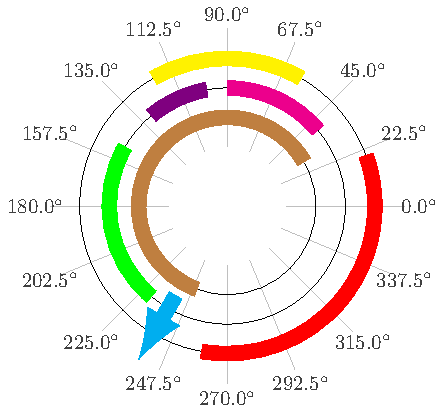
\includegraphics[width=\linewidth]{Winkelbereiche_einzelner_Vorgaenge_Picture}
\end{minipage}

\caption{Winkelbereiche einzelner Vorgänge während eines Maschinentaktes}\label{fig:Winkelbereiche einzelner Vorgaenge}
\end{figure}








\subsection{Synchrone Bewegungen}

Die Bewegungsabläufe im Produktionsprozess wiederholen sich in periodischen Zyklen. Die Steuerung der Bewegungen bei den rein mechanisch gesteuerten Maschinen erfolgt über Kurvenscheiben. Weil diese mechanisch gekoppelt sind, werden alle Bewegungen von dem zentral antreibenden Motor zwangsgesteuert. So entsteht eine zum Hauptantrieb synchrone Bewegung. Für die elektronisch gesteuerten Maschinen ist die synchrone Bewegung wie folgt definiert:

\blockquote{Die Achse führt eine Bewegung aus, die Drehzahl- und Winkelgleich zu einem zugeordneten Drehgeber der Anlage erfolgt.} \cite{OttoBihlerMaschinenfabrikGmbH&Co.KG2015}

In der VC 1 Maschinensteuerung ist ein elektronischer Drehgeber hinterlegt, der die zentrale Ansteuerung aller anderen Bewegungen übernimmt. Die einzelnen Bewegungsabläufe sind als Cams einprogrammiert worden (vgl. Kapitel~\ref{cha:Bewegungsprofile und Bewegungsablauf}).




% Zur Darstellung der unterschiedlichen Bewegungsabläufe in einem Zyklus wird auf einen Kreis mit \SI{360}{\degree}zurückgegriffen.  Die  Zeiträume  der  einzelnen  Bewegungen  können  in  Winkelgrade umgerechnet und veranschaulicht werden. Dieses Konzept ist als Kurvengetriebe bekannt.







\subsection{Asynchrone Bewegungen}\label{cha:Asynchrone_Bewegung}

Laut Betriebsanleitung der VC 1 ist eine asynchrone Bewegung wie folgt definiert:

\blockquote{Die Achse führt eine Bewegung aus, die zu einem bestimmten Zeitpunkt gestartet wird, und dann mit vorgegebenen Profil und festgelegter Geschwindigkeit ausgeführt wird.} \cite{OttoBihlerMaschinenfabrikGmbH&Co.KG2015}

Im Gegensatz zu den Bewegungsabläufen bei den mechanisch zwangsgesteuerten Kurvenscheiben, die einem periodischen Zyklus unterliegen, besteht bei den rein elektrisch angetriebenen NCAs die Möglichkeit, Bewegungen auch völlig unabhängig von einem Drehgeber auszuführen. So kann z.B. auf ein Signal hin eine komplette Bewegung ausgeführt werden, ohne dass der Drehgeber der Anlage darauf einen Einfluss hat, weshalb man von einer asynchronen Bewegung spricht.



Im Gegensatz zu den synchronen Bewegungen kann bei asynchronen Bewegungen ein so genanntes Trapezprofil (vgl. Kapitel~\ref{cha:Trapez und Dreiecksprofil}) benutzt werden. Das heißt, wenn die Achse mit einem Trapezprofil betrieben werden soll, muss die Achse über eine asynchrone Bewegung angesteuert werden, denn mit der VC 1 Steuerung kann im Synchronbetrieb kein Trapezprofil verwendet werden.


Eine große Gefahr geht im Einrichtbetrieb, der die Maschine auf den Automatikbetrieb vorbereitet, von den asynchronen Bewegungen aus. Da die asynchronen Bewegungen nach dem Erhalt eines Eingangssignals mit der Ursprungsgeschwindigkeit gestartet werden und dann mit der programmierten Geschwindigkeit ablaufen, passen sie sich im Gegensatz zum Synchronbetrieb, bei dem die Bewegungen mit dem Drehgeber der Anlage gekoppelt sind, nicht an die verlangsamte Geschwindigkeit des Einrichtbetriebs an.
